\documentclass{article}
\usepackage{fullpage}
\usepackage{graphicx}
\usepackage{caption}

\captionsetup{font=scriptsize,labelfont=scriptsize}


\author{Fergus W. Leahy - 0908622L}

\title{Wireless Sensor Networks Assessed Coursework 2}

\begin{document}
\maketitle{}

\section{Introduction}
The purpose of this report is to discuss the design and implementation of the Twitter-like framework, Tinyblog, for the wireless sensor devices, as well as demonstrate the extent to which the requirements have been fulfilled.  

\section{Design}
The design of the TinyBlog framework is tightly bound by the modularity of TinyOS, where possible the implementation has been split into modules (such as Packet buffers).

Figure \ref{fig:modules} shows the basic wiring of different modules in the system. A full diagram of the wiring can be found in the appendicies.
\begin{figure}[htb!]
\centering
\includegraphics[scale=0.4]{TinyBlog_wiring.jpg}
\caption{TinyBlog wiring}
\label{fig:modules}
\end{figure}  

The system modules include: 
\begin{itemize}
	\item Active messaging - used to communicate over the radio
	\item Light/Temp sensors - used to create mood data
	\item Timers - used for various tasks which must be triggered repeatedly, such as retrieving sensor readings for the mood
	\item LEDS - used to signify activity on the network, i.e., blink red for tweet forwarded
\end{itemize}

The TinyBlog modules include:
\begin{itemize}
	\item Follow List(Circular Queue) - used to store the users which the node is following
	\item Packet Buffer - used to store the metadata (src, seqno) of recent packets received (to stop broadcast storm)
	\item Tweet Queue - used to store the messages of tweets received or ready to transmit on the network(depending of scenario).
	\item Interest Table - used to create a cache of any recently seen interests for tweets(used for scenario 2).
\end{itemize}


\section{Requirements fulfilled}
\subsection{Transferred data format}
\begin{itemize}
	\item Use of specified data format - TinyBlogMsg.h has been included and used where necessary
	\item Message body of 100 bytes - DATA\_SIZE has been modified to 100 bytes and TOSH\_DATA\_LENGTH is set through a compile time flag to accommodate the extra bytes
	\item End of message - The host application automatically truncates a message which is too long and sets nchars to the correct number of chars.
\end{itemize}

\subsection{Host-side Application}
The host-side application is a command line application written in Java, this was chosen due to the familiarity of the author with Java, as well the documentational support and examples of how the application should be created.

\begin{itemize}
	\item Client communicates to the mote application via the base station
	\begin{itemize}
		\item the application allows users set the destination of their actions to their specific node, this is done by calling, \textit{connect} \textless nodeid\textgreater
	\end{itemize}
 	\item Allow users to post tweets
 	\begin{itemize}
 		\item the application allows users to post tweets to the node which it is connected to.
 	\end{itemize}
 	\item Allow users to follow tweets from other users
 	\begin{itemize}
 		\item The host-side application allows a user to indicate which nodes to follow for tweets, using the command: \textit{follow} \textless nodeid\textgreater, where nodeid is the node the user wants to follow. This is then sent as a message to the mote application which then updates its follow list. After which it will then save any messages which it receives if the mote ids are in the list.
 	\end{itemize}
 	\item Poll the state of the buffer
 	\begin{itemize}
 		\item The host-side application can request all the tweets the node has received, these are displayed on the host-side application.
 	\end{itemize}
 	\item Receive a message from someone followed and display on client
 	\begin{itemize}
 		\item When a new message has arrived on the node, after it is processed it is then saved and transmitted the the base station where the host-side application receives and displays the tweet. 
 	\end{itemize}
 \end{itemize} 


\subsection{Mote application}
\begin{itemize}
	\item LED actions
	Several led actions have been implemented to make it easier to understand the activity of the mote from the onboard leds. Actions with signify positive activity have relatively short LED blinks, 2Hz, where as actions with signify negative activity (dropped packet/problem) have relatively long LED blinks, 1Hz. The reason for this was to make it easier to see when problems occur on the mote, which should hopefully be less frequent, hence the longer blinks would make it easier to see when they do occur.
	\begin{itemize}
		\item Get tweet, blink blue, 2Hz
		\item Post tweet, blink green, 2Hz
		\item Forward tweet, blink red, 2Hz 
		\item Receive message, blink red \& green, 5Hz
		\item Send message, blink greed, 5Hz
		\item Dropped message, blink red, 1Hz
		\item Problem, blink red \& green \& blue, 1Hz
	\end{itemize}
	\item Multi-hop, packet forwarding
	\begin{itemize}
		\item The mote application fully supports robust packet forwarding and avoids contributing to broadcast storms. This is done through the correct use of using the TTL field in the data structure, as well as using a buffer of previously seen packet meta data. This buffer is used so that when new packets arrive they can be checked and if a match is found in the buffer they are dropped immediately, as they must have been re-broadcasted. The buffer is a circular data structure storing 32 packets metadata, so when full it overwrites the oldest packet. This makes a compromise between the size of the buffer and the amount of ``recent'' packets which can be recognised.
	\end{itemize}
	\item Support Minimal Protocol commands
	\begin{itemize}
		\item All minimal commands have been implemented and depending on the scenario the functionality changes.
		\begin{itemize}
			\item Post tweet
			\begin{itemize}
			 	\item In scenario 1, when a post tweet is received from the base station, the mood and source mote id is set, and then the tweet is broadcast across the network. If a mote receives a new, unseen post tweet from a mote which is mote which is not the base station then it checks if it is follow the user which created it, if so it saves it locally and then transmits it to the base station. Regardless of whether the tweet was followed, it is broadcasted back on to the network if it has not expired its TTL.
			 	\item In scenario 2, when a post tweet is received from the base station it is just stored locally on the mote, waiting for a get tweet message from another mote. If it receives a post tweet message from another mote on the network it checks to see if it can route it, (further discussed in the \ref{sec:dd}), if so then it sends it to the next hop.
			\end{itemize} 
			\item Add user to follow list
			\begin{itemize}
			 	\item In both scenarios, when the host side applications sends a follow user message to the mote, the mote stores the id in its follow list. This follow list is then consulted when either receiving tweets or looking for tweets. 
			 \end{itemize} 
			 \item Retrieve new tweets
			 \begin{itemize}
			 	\item In scenario 1, when the host-side application sends the get tweets command, the mote sends all of the tweets stored in its local cache back to the host.
			 	\item However, in scenario 2 the mote does not store the tweets locally, so instead it sends an get tweets request to other motes which it follows (an interest).
			 \end{itemize}
		\end{itemize}

	\end{itemize}
\end{itemize}

\subsection{Scenarios}
Both scenarios have been implemented and can be selected at compile time by specifying the -DSCEN=N flag in the makefile, where N is the scenario number.
\subsubsection{Scenario 1}
Scenario 1 has been fully implemented with the appropriate forwarding mechanics as set by the specification.

\subsubsection{Scenario 2}
\label{sec:dd}
Scenario 2 has been implemented with directed-diffusion based routing. This is implemented using the concept of interests (get tweet), events (post tweet) and an interest cache. When a mote issues a get tweet request it broadcasts it to the network, each mote that receives this checks if it has already seen this request in its interest cache, if not then it creates an entry storing the destination of the request and previous hop address. However if it has already seen this request then, it has either come from another route, possibly worse/slower, and so it is ignored. It then broadcasts the get tweets request to its neighbours, this is repeated until the destination mote receives the request. Once received it then sends its tweets back the direction the request came from, each mote that receives it then checks its interest table for the next hop based on the source of the event (the destination of the get tweet/interest). If any mote sees the data more than once, it drops the packet. Routes are also erased if they are not refreshed from repeat request after a short period of time.

\subsection{Additional Requirements}
\subsubsection{Mood}
Capturing the mood by sensing the temperature and light readings from the user's mote has been implemented. It has been implemented by using a periodic timer which senses the temperature and light intensity every 5 seconds, so when the user sends a tweet the most recent mood data, up to 5 seconds old, is attached to the tweet. This was done because of the split-phase nature of the sensors, by using a timer and then copying the most recent readings into a tweet means that the system doesn't have to wait for the sensors to signal an event to continue the tweeting.
If the platform does not have sensors available, the -DTELOS flag can be removed and instead the DemoSensor module will be used.
\subsubsection{Updateable follow list}
The follow list which is stored in the mote is fully updateable at run-time. This is done by sending a \textit{follow} command from the host-side application to the users mote, where it adds the mote id to a follow list. If too many ids are added, the list overwrites the oldest id (circular queue).
\subsubsection{Direct messaging}
Direct messaging to specific motes has been implemented in both the host-side and mote applications. To send a direct message the command is: \textit{direct} \textless nodeid\textgreater message .
The message is then unicast directly to the mote specified, once the mote receives it the message is then forwarded to the base station where it is displayed by the host-side application. For this an extra action, was created in TinyBlogMsg.h.
\subsubsection{Encryption}
Encryption of tweets has been enabled as a compile time option, -DSECURE \& -DCC2420\_HW\_SECURITY, also included in the BaseStation folder is the encrypted enabled Base station to communicate with the motes. It has been implemented using the encryption capabilities of the CC2420 radio onboard the TelosB motes and uses the SecAMSender module to encrypt and send the messages. For receiving packets, the normal AMReceiver module handles decryption of the messages and simply returns the same payload as if it were unencrypted. All nodes use the same key to encrypt and decrypt the data.
The implemented version, Counter Mode Encryption (CTR), only supports encryption of the data, but modifying the implementation to use both encryption and authentication would be relatively straight forward by using Counter with Cipher Block Chaining Authentication Code (CCM) instead. By doing so it would allow the motes to ensure that the data being transmitted is secure and that it is from who it says it's from. 


\section{Testing \& Evaluation}
\subsection{Scenario 1}
For testing scenario 1, three TelosB motes were used, one as a base station and two as user motes. Both motes used the same base station to talk to the host-side application. The follow section shows a step by step view of sending a receiving tweets.

Figure \ref{fig:tweeting} shows the user connecting to a specific mote, adding a new user to their follow list, and then for demonstrational purposes connecting to the followed mote and tweeting from it. In figure \ref{fig:motetweeting} the users mote shows how it reacts to incoming tweet messages and recognises the different actions it needs to perform, where 0 is the base station, 1 and 3 are the user motes, and -1 is everyone on the network.
\begin{figure}[htb!]

\begin{minipage}{.5\textwidth}
\begin{center}
    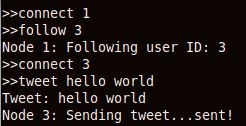
\includegraphics[scale=.6]{img/tweet.jpg}
    \centering
	\captionof{figure}{Connecting to a user mote, following a user and sending a tweet}
	\label{fig:tweeting}
	\end{center}
    \end{minipage}%
    \begin{minipage}{.5\textwidth}
    \begin{center}
    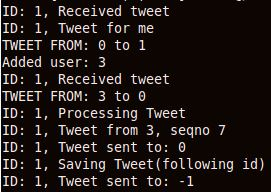
\includegraphics[scale=.5]{img/motetweet.jpg}
    \captionof{figure}{Mote side application \\receiving commands}
    \label{fig:motetweeting}
\end{center}

\end{minipage}

\end{figure}

Because mote 1 followed mote 3, as soon as a tweet is received on mote 1 whose user exists in the follow list, the tweet is forwarded to the base station to be displayed by the host-side application, as shown in figure \ref{fig:receive}.
\begin{figure}[htb!]
\centering
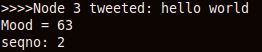
\includegraphics[scale=.7]{img/receive.jpg}
\caption{Receiving a tweet from a followed user}
\label{fig:receive}
\end{figure}

\newpage
As one of the requirements implementing long tweets (\textless101 chars) is necessary and as show in figure \ref{fig:long} it works.
\begin{figure}[htb!]
\centering
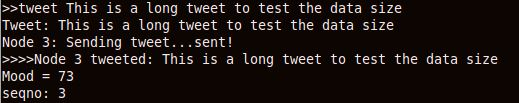
\includegraphics[scale=.50]{img/long.jpg}
\caption{Sending a long tweet}
\label{fig:long}
\end{figure}


Lastly the ability to a later time retrieve all followed tweets is necessary, so when the user types: \textit{get} into the host-side application the user's mote returns all messages the follow motes have tweeted, shown in figure \ref{fig:get}.
\begin{figure}[htb!]
\centering
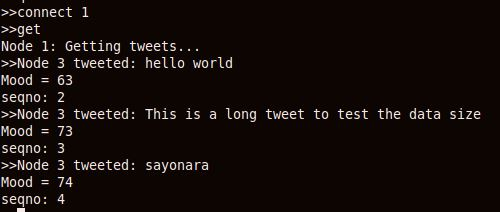
\includegraphics[scale=.6]{img/get.jpg}
\caption{Fetching tweets for users followed}
\label{fig:get}
\end{figure}


\subsection{Scenario 2}


\newpage
\section{Appendices}
\begin{figure}[htb!]
\centering
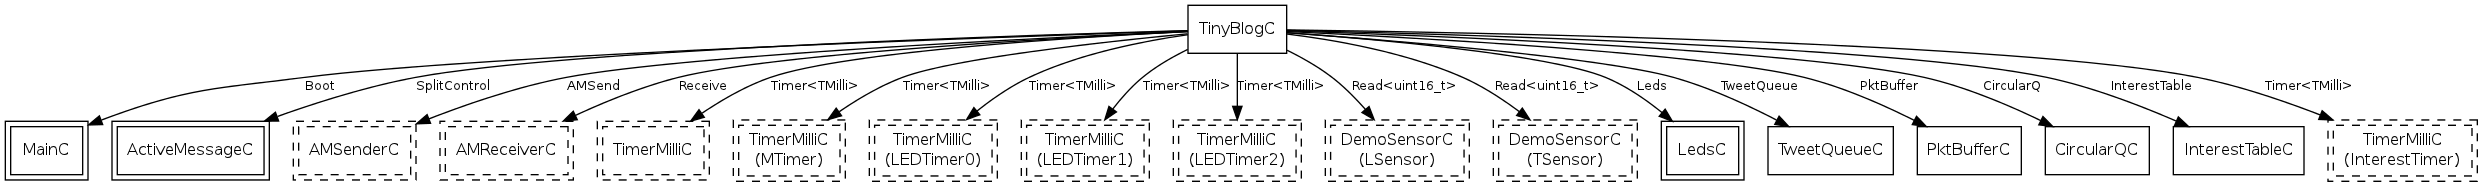
\includegraphics[scale=.27,angle=90]{TinyBlogAppC.png}
\caption{TinyBlog wiring, created using nesdoc}
\label{fig:fullWiring}
\end{figure}



\end{document}